\chapter{$b$-jet Triggers}\label{appendix:bjet_trigger}

\section{Parsing Trigger Chains}\label{section:trigger_chain_names}

Trigger algorithms (known as ``chains'' as they are a series of criteria and algorithm decisions) are complex series of logic.
Their naming conventions are not readily clear to the uninitiated, so the following is a very brief summary of how to parse the grammar of $b$-jet triggers (for more detail c.f.~\cite{Feickert:HbbWorkshop2017}). An example chain name in COMA~\cite{TWiki:ConditionsMetadata,COMA:ChainReport}, \texttt{\textcolor{black}{HLT}\_\textcolor{red}{j55}\_\textcolor{green}{gsc75}\_\textcolor{blue}{bmv2c1040}\_\textcolor{purple}{split}\_\textcolor{red}{3j55}\_\textcolor{green}{gsc75}\_\textcolor{orange}{boffperf}\_\textcolor{purple}{split}}, is decomposed below.
\begin{itemize}
 \item \texttt{\textcolor{black}{HLT}}: HLT trigger chain prefix to distinguish from L1 items.
 \item \texttt{\textcolor{red}{nj55}}: Requires at least $n$ jets with $p_{T} > 55~\GeV$.
 \item \texttt{\textcolor{purple}{split}}: \texttt{superROI} configuration being used for 2-step track reconstruction and primary vertex finding.
 \item \texttt{\textcolor{green}{gsc75}}: Apply Global Sequential Corrections (GSC) to jets passing first $p_{T}$ threshold and require jets with GSC $p_{T} > 75~\GeV$.
       \begin{itemize}
        \item GSC requires track reconstruction to be run, but as $b$-tagging requires tracking there is no extra cost in $b$-jet trigger chains.
       \end{itemize}
 \item \texttt{\textcolor{orange}{boffperf}}: The $b$-tagging algorithm (\texttt{MV2c10}) is run over the jets but no selection is applied on the output.
 \item \texttt{\textcolor{blue}{bmv2c1040}}: Requires passing the \texttt{MV2c10} $b$-tagging algorithm at the $40\%$ selection efficiency working point.
\end{itemize}

The result is that the trigger chain name should be parsed to read ``at least 4 jets with GSC $p_{T} > 75~\GeV$ and track reconstruction and primary vertex finding done using Super-RoI configuration to have had \texttt{MV2c10} $b$-tagging algorithm run over them, and at least 1 of them to have passed the \texttt{MV2c10} $b$-tagging algorithm at the 40\% selection efficiency working point.''


\section{Super-RoIs}\label{section:super-RoI}

The purpose of the $b$-jet trigger to provide effective $b$-jet identification and light-jet and $c$-jet rejection in the \gls{HLT} to maximize the number of interesting physics events containing heavy flavor physics.
This still needs to be done quickly, but given that $b$-tagging is being performed on each jet candidate that passes other selection criteria tracking must also be performed.
As a result, the $b$-jet triggers are the leading consumers of CPU out of all triggers in the ATLAS trigger menu.
In Run 2 to address this issue a new CPU and time saving measure was introduced~\cite{Hetherly:2313140}.
Instead of running the track matching algorithms in each \gls{RoI} that existed for the event, even if there was substantial overlap between the RoIs, all RoIs --- regardless of if they have topologically overlap --- are merged into a single ``Super-RoI,'' as seen in \Cref{fig:all_ROI_vs_superROI}.
Once the Super-RoI has been created, fast tracking is run in the Super-RoI to find a primary vertex.
Once a primary vertex has been found, precision tracking is then run in each of the original RoIs, but with the tracks constrained by the Super-RoI primary vertex.

\begin{figure}[htbp]
 \centering
 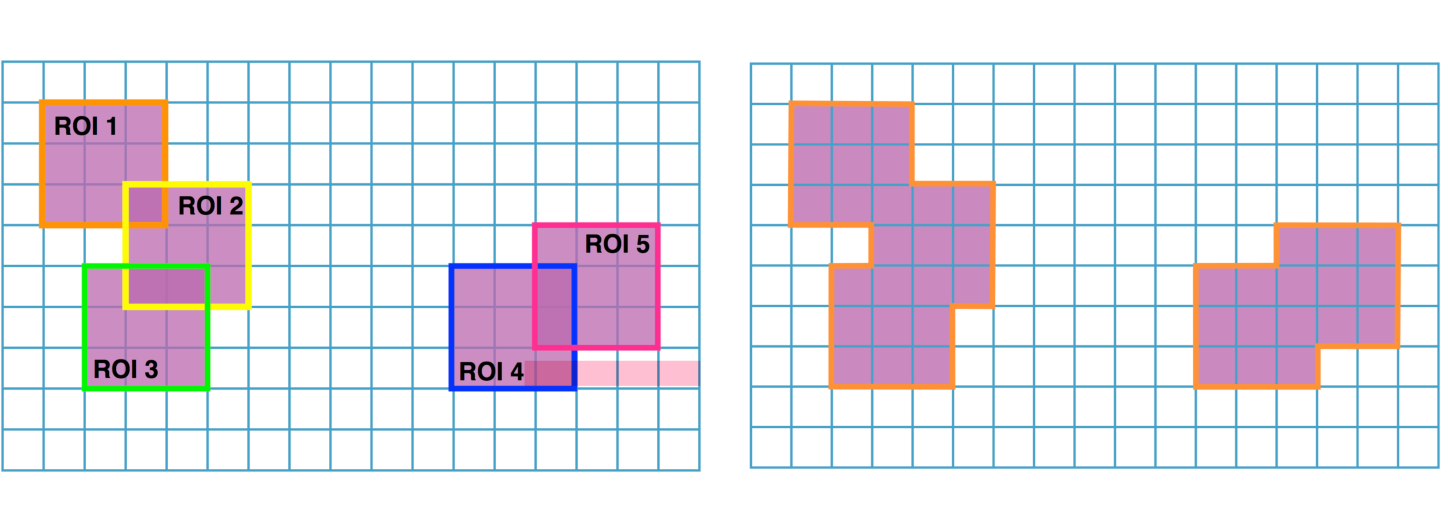
\includegraphics[width=\textwidth]{appendix/all_ROI_vs_superROI.pdf}
 \caption[Cartoon of the all RoI vs. the Super-RoI configuration for tracking run by the $b$-jet trigger.]{%
  Cartoon of the all RoI (no-split) configuration (left) vs. the Super-RoI (split) configuration (right) configuration for tracking run by the $b$-jet trigger.
  The gird represents $\eta$-$\phi$ space.
  The Super-RoI may not be topologically connected but counts as a single object~\cite{Hetherly:2313140}.}
 \label{fig:all_ROI_vs_superROI}
\end{figure}

\section{$b$-jet Trigger Efficiency in High Pile-up}\label{section:BJetTrig_efficiency}

As the LHC moves into Run 3 the energy and luminosity will increase, causing there to be higher pile-up, as discussed in \Cref{section:LHC_collider}.
To characterize the performance of the 2017 $b$-jet trigger chains in these future environments I performed a study of the $b$-jet trigger efficiency in high pile-up environments using high purity di-lepton $t\bar{t}$ events in the 2017 data-set to provide a sample enriched with $b$-jets.
The results, seen in \Cref{fig:BJetTrigg_efficiency_vs_mu} and \Cref{fig:BJetTrigg_pass_fraction_vs_mu}, show that the $b$-jet triggers compared to the offline $b$-tagging algorithm \texttt{MV2c10} at the $70\%$ efficiency operating point have a high and flat efficiency for pile-up, $\braket{\mu}$, out to beyond $\braket{\mu}=60$.
Likewise, the number of jets that pass the online $b$-tagging requirement remains proportionally low given the different efficiency operating points.
Beyond $\braket{\mu}=60$ there starts to be some degradation for the lower online efficiency operating points, though the statistical uncertainty also begins to increase.
The plots to not extend out to $\braket{\mu}=70$ as there was insufficient number of events to have reasonable statistical uncertainties given the dataset used.
Similar results were obtained when the study was repeated using 2018 triggers and data~\cite{Sekula:2631805}.

\begin{figure}[htbp]
 \centering
 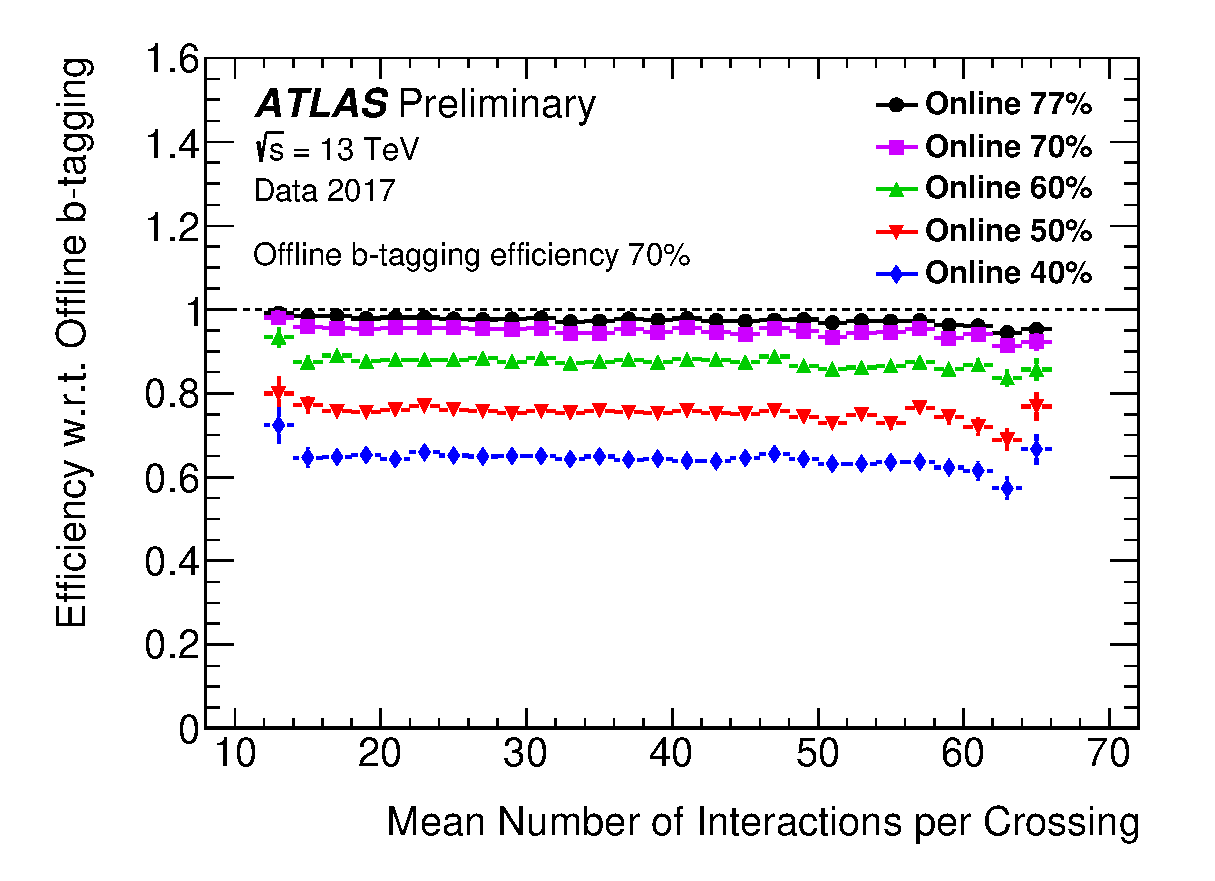
\includegraphics[width=\textwidth]{appendix/BJetTrigg_efficiency_vs_mu.eps}
 \caption[The $b$-jet trigger efficiency with respect to the offline $b$-tagging algorithm (\texttt{MV2c10}) at the 70\% efficiency operating point for various online efficiency operating points vs. the mean number of interactions per crossing.]{%
  The $b$-jet trigger efficiency with respect to the offline $b$-tagging algorithm (\texttt{MV2c10}) at the 70\% efficiency operating point for various online efficiency operating points vs. the mean number of interactions per crossing.
  The relative $b$-jet trigger efficiency is measured in high purity di-lepton $t\bar{t}$ events collected in the 2017 data-set using dedicated single-lepton$+$jets triggers, which are unbiased with respect to the online $b$-tagging.
  The online operating points were defined to have roughly the quoted efficiency for $b$-jets in an unbiased sample of Monte Carlo simulated $t\bar{t}$ events.
  The uncertainty bars shown only represent statistical uncertainties~\cite{Feickert:2294576}.}
 \label{fig:BJetTrigg_efficiency_vs_mu}
\end{figure}

\begin{figure}[htbp]
 \centering
 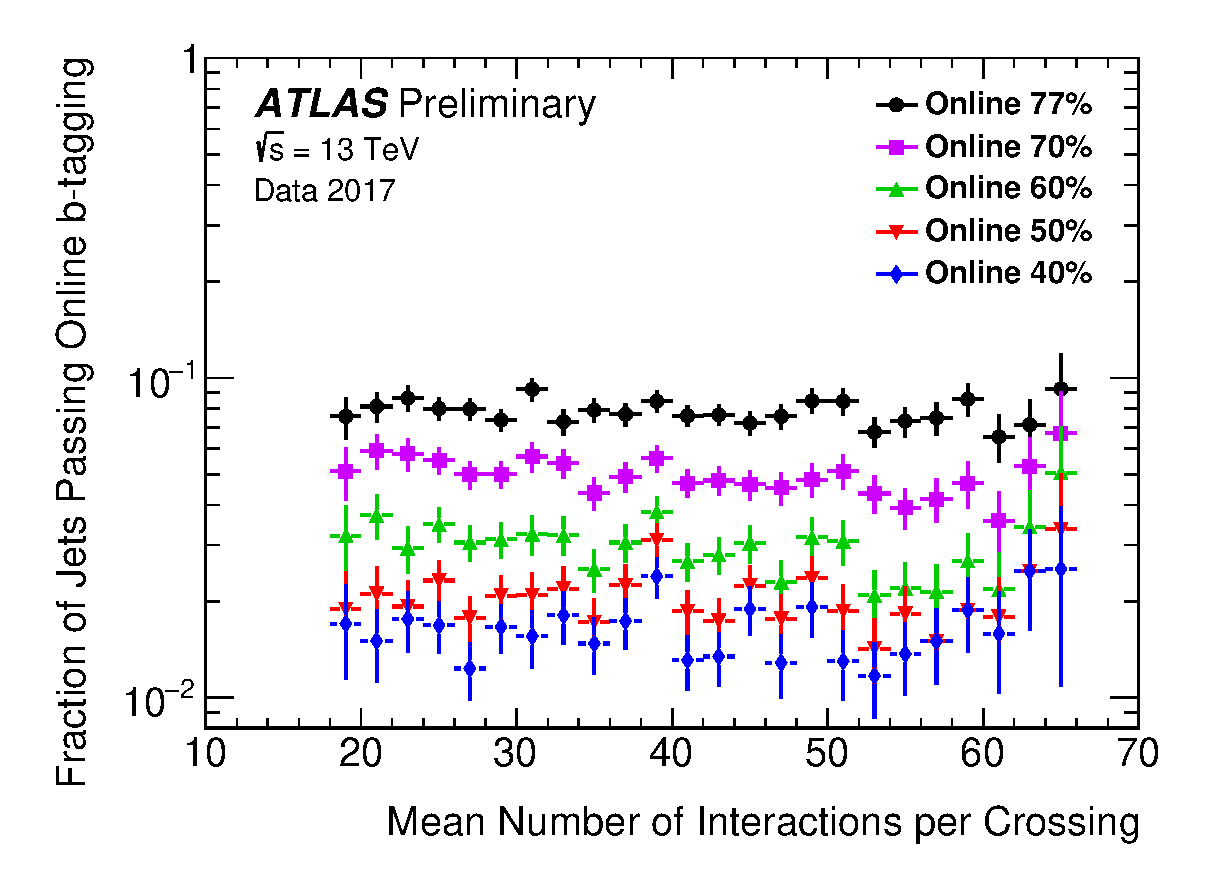
\includegraphics[width=\textwidth]{appendix/BJetTrigg_pass_fraction_vs_mu.eps}
 \caption[The fraction of trigger jets with Global-Sequential-Calibration-corrected $E_T > 55~\GeV$ that pass the online $b$-tagging algorithm (\texttt{MV2c10}) at various online efficiency operating points vs. the mean number of interactions per crossing.]{%
  The fraction of trigger jets with Global Sequential Calibration (GSC)-corrected $E_T > 55~\GeV$ that pass the online $b$-tagging algorithm (\texttt{MV2c10}) at various online efficiency operating points vs. the mean number of interactions per crossing.
  The pass fraction is measured in a subset of the 2017 data-set with events containing at least one jet with GSC-corrected $E_T > 55~\GeV$.
  The trigger used is unbiased with respect to the online $b$-tagging.
  The online operating points were defined to have roughly the quoted efficiency for $b$-jets in an unbiased sample of Monte Carlo simulated $t\bar{t}$ events.
  The uncertainty bars shown only represent statistical uncertainties~\cite{Feickert:2294576}.}
 \label{fig:BJetTrigg_pass_fraction_vs_mu}
\end{figure}
